\documentclass[a4paper, 12pt]{book}
\usepackage{amsmath}
\usepackage{amsfonts}
\usepackage{amssymb} 
\usepackage{centernot}
\usepackage{verbatim}
\usepackage{graphicx}
\usepackage[colorlinks]{hyperref}
\usepackage{caption}
\usepackage{subcaption}
\usepackage{titlesec}	
\usepackage{scrextend}
\usepackage{titlepic}
\usepackage{float}
\usepackage{wrapfig}
\usepackage{lscape}
\usepackage{rotating}
\usepackage{epstopdf}
\usepackage{pdflscape}
\usepackage{ulem}
\usepackage[margin=0.8in]{caption}
\usepackage[margin=0.8in]{geometry}
\usepackage{array,multirow,multicol}
\begin{document}


We nevertheless consider an alternative approach to define the dynamic of nodes leaving the work queue and joining the worker pool that both prevents Sybil attack and incentivise nodes to join the work queue during periods of low demand for work.

We propose a method to sort out the nodes listed in the worker queue. A ranking (or score) is associated to a node when it joins the work queue. The nodes in the worker queue are then ordered based on their ranking in descending order, \textit{i.e.} the nodes with the lowest ranking are at the top of the queue and the first ones to leave the work queue and be selected to join the worker pool when some slots are freed in the worker pool. The method to assign a ranking to a node joining the worker queue is not purely chronological-based. It depends on the volume of nodes joining the queue during same allotted time period $\Delta t$. Assume $S_t$ nodes applying to join the worker queue during a small window of time $[t, t+\Delta t]$. The $S_t$ nodes first register to a tertiary queue, $DHT_s$. At the end of the time window, a fixed and limited number of nodes from $DHT_s$, $z \leq S_t$, are randomly selected. $z$ is equal to the number of nodes who left the worker pool during the time window  $[t-\Delta t, t]$. These $z$ nodes are given a ranking drawn from a normal distribution centred around $R_q$, which is a predetermined threshold of the worker queue length. This means that some selected nodes may obtain a ranking higher than nodes currently at the bottom of the worker queue. The rest of the nodes in the tertiary queue ($S_t-z$) are given a ranking drawn from a normal distribution centred around $R_l = R_q - s$, where $s$ is a shift inversely proportional to the volume of nodes in the tertiary queue $DHT_s$. Figure~\ref{fig:NSM} illustrates the process of ranking allocation for nodes joining the worker queue. \\

In the example given in the figure below, for time $t$, $z = 3$ as this is the number of nodes that leave $DHT_w$ at the end of the time period $t$. $z$ can thereby be represented by $A$, $B$ and $C$ which move into $DHT_q$ with a normal score at $t + \Delta t$. $D$ therefore is in the remaining nodes in $S_t - z$ that enter $DHT_q$ with a low score. $z$ for the time period $t + \Delta t$ is 5 as this is the number of nodes that leave $DHT_w$ at the end of the time period $t + \Delta t$. Thereby 5 nodes will join $DHT_q$ with a high score at time $t + 2\Delta t$.

\newpage
\begin{landscape}
\begin{figure}
\centering
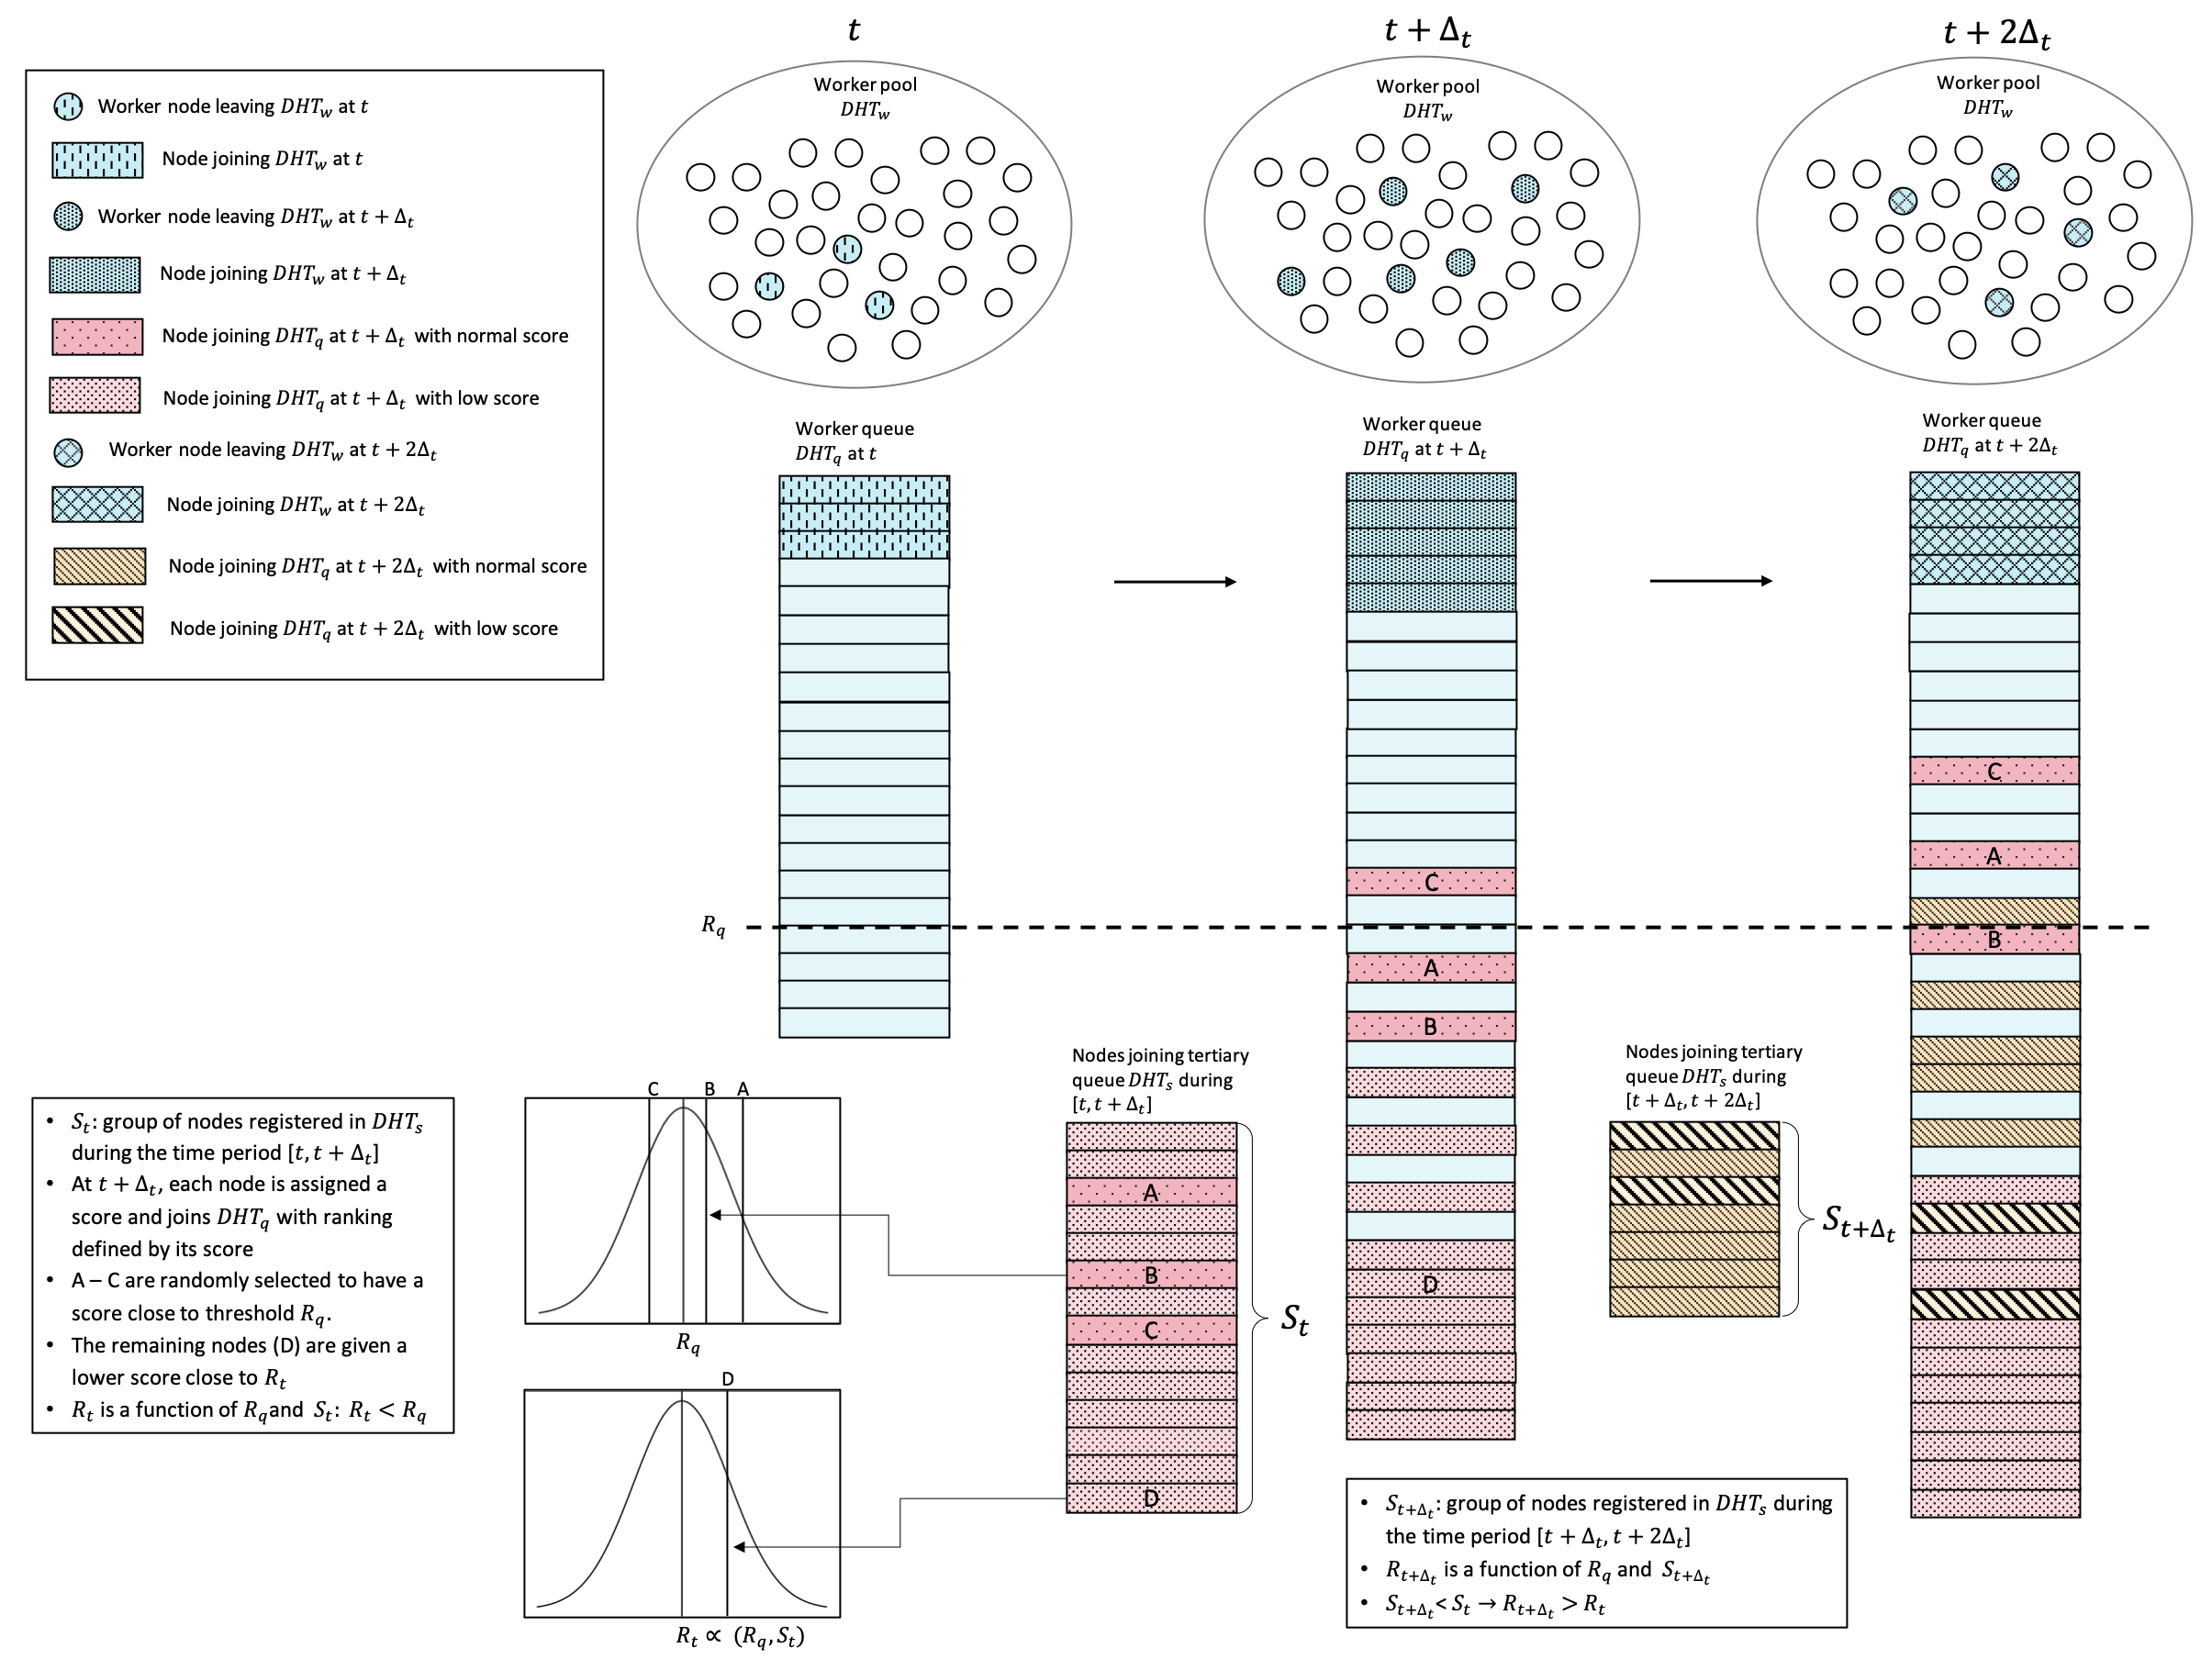
\includegraphics[width=22cm,height=42cm,keepaspectratio]{Work_Queue_Management}
\caption{\label{fig:NSM}Illustration of the process followed by Catalyst network to add nodes to the work queue.}
\end{figure}
\end{landscape}

\end{document}
